\section{Reconstruction of Collision Events in the ATLAS Detector}%
\label{sec:object_reco_at_atlas}

\todo[inline]{Introductory sentence}

Omissions: Photons, special reconstruction techniques for certain analyses


\subsection{Tracking and Vertexing}

The reconstruction of trajectories of charged particles is referred to as track
reconstruction or tracking. The inputs to the track reconstruction in the ID of
the ATLAS detector are \emph{space-points} from the pixel and SCT detector, and
\emph{drift circles} from the TRT. Space-points are measurements of location in
three-dimensional space obtained by clustering the charge signals of adjacent
segments in the pixel and SCT detectors. Drift circles are measurements of
distance from the anode wires of individual straw-tubes in the TRT derived from
electron drift times in the straw-tubes.

Track reconstruction employs pattern recognition techniques to select
space-points and drift circles that are compatible with the hypothesis of a
charged particle in the axial magnetic field of the ID. Least-squares fits are
performed, using selected space-points and drift circles, to determine the
parameters characterising the track at a reference point. This reference point
is typically the point of closest approach (perigee) to the nominal beamspot
position in the transverse plane. Five parameters describe the track at the
perigee. The transverse (longitudinal) distance of the perigee from the
reference point given by $d_0$ ($z_0$), also referred to as the transverse
(longitudinal) impact parameter of the track. The azimuthal and polar angle of
the track at the perigee given by $\phi$ and $\theta$, respectively. Finally,
the ratio of electric charge and transverse momentum, $q / \pT$, parameterises
the curvature of the track.

At the ATLAS experiment, two primary tracking algorithms are used which are
referred to as the \emph{inside-out} and \emph{outside-in}
algorithms~\cite{Cornelissen:2007vba,Salzburger:2015sgq,PERF-2015-08}. The
inside-out algorithm starts by reconstructing tracks in the pixel and SCT
detector only, then extending the track using measurements in the TRT. In
contrast, the outside-in algorithm starts with the reconstruction of track
segments in the TRT which are them combined with space-points from the pixel and
SCT detectors. The outside-in algorithm is used to improve the reconstruction
efficiency for tracks from secondary particles, such as electrons produced in
conversions of photons in the detector material, for which the inside-out
algorithm can fail to reconstruct a track.

Reconstructed tracks are used to determine the locations of inelastic scattering
interactions between protons in the ATLAS detector. These locations are marked
by multiple charged particle tracks originating from the same point in the
detector and are referred to as primary vertices (PVs). Consequently, the vertex
of the hard scattering interaction of interest and the associated particles can
be identified, allowing to reject reconstructed objects originating from
pile-up. The ATLAS primary vertex reconstruction~\cite{PERF-2015-01} finds and
reconstructs PVs using an iterative fitting procedure. The PV reconstruction
starts by reconstructing a vertex at the location of highest track density in
$z_0$ with respect to the beamspot position. An adaptive vertex
fitter~\cite{Fruhwirth:2007hz} is used to iteratively determine the vertex
position while weighting reconstructed tracks according to their compatibility
with the vertex position. After the fit, tracks that are incompatible with the
vertex position are considered as unassociated and the process is repeated on
all unassociated tracks. Finally, the PV with the largest sum of $\pT^2$ of
associated tracks that has at least two tracks with $\pT > \SI{500}{\MeV}$ is
selected as the PV of the hard scattering interaction of primary interest. Other
vertices with at least two associated tracks are considered as originating from
pile-up~\cite{PERF-2015-01}.


\subsection{Topological Clustering of Energy in Calorimeter Cells}

The segementation of the calorimeters in lateral and longitudinal direction
allows to reconstruct the three-dimensional shape of electromagnetic and
hadronic showers. These showers typically extend over multiple cells in the
calorimeter, thus requiring the combination of several cells to fully
reconstruct a shower. The ATLAS experiment uses a \emph{topological calorimeter
  cell clustering algorithm}~\cite{PERF-2014-07} to combine the signals of
locally connected cells passing certain signal thresholds, thereby suppressing
noise from the calorimeter electronics and pile-up. These clusters of
calorimeter cells, referred to as topo-clusters, are used to reconstruction
electromagnetic and hadronic showers in the calorimeters. Due to fluctuations in
the shower development, multiple topoclusters are typically required to fully
reconstruct the calorimeter response to a single particle.

The ATLAS calorimeter has a different response to electromagnetic and hadronic
showers, i.e.\ the calorimeter is \emph{non-compensating}. By default, the
energies of topoclusters are calibrated assuming the response originates from an
electromagnetic shower (EM scale). However, the development of electromagnetic
and hadronic showers leads to differences in their shower shapes, as previously
discussed in \Cref{sec:atlas_calorimeters}. This is exploited by the \emph{local
  hadronic calibration}~\cite{PERF-2014-07} which uses shape information of
individual topoclusters to determine their likely origin and apply
electromagnetic and hadronic calibrations that are weighted accordingly. The
energy scale of topoclusters after the local hadronic calibration is referred to
as the LC scale.

Topoclusters are used as inputs for the reconstruction of higher-level physics
objects in the ATLAS detector. For example, topoclusters at EM and LC scale are
used in the reconstruction of jets and \tauhadvis, respectively, which is
discussed in \Cref{sec:jet_rec,sec:tau_rec}.


\subsection{Electrons}%
\label{sec:ele_rec}

The reconstruction of electrons (and positrons) in the ATLAS detector exploits
their characteristic signature of a charged particle track pointing towards a
narrow cluster of energy in the electromagnetic calorimeter. The reconstruction
of electrons in the region of $|\eta| < 2.47$ based on
Refs.~\cite{ATL-PHYS-PUB-2017-022,EGAM-2018-01} is described in the following.

Electron reconstruction is seeded by topo-clusters that have more than
\SI{50}{\percent} of their energy located in cells of the electromagnetic
calorimeter (EM topo-clusters). In addition, topo-clusters are only considered
if the transverse energy in the electromagnetic part of the calorimeter,
$\ET^{\text{EM}}$, exceeds \SI{400}{\MeV}. A first attempt of geometrically
matching the EM topo-cluster to an ID track is made. If the EM topo-cluster
cannot be matched to a well-reconstructed track but has a longitudinal and
lateral shower shape similar to the signature of an electron, then a second pass
of tracking is performed in a region surrounding the cluster. The second pass
allows for up to \SI{30}{\percent} of energy loss at each intersection with
detector material due to the emission of bremsstrahlung. After an ambiguity
resolution scheme in case multiple tracks match the cluster, the cluster is
required to be geometrically matched to a single track. EM topo-clusters with
matched tracks are considered as seeds for a \emph{supercluster} reconstruction
algorithm if the cluster fulfils $\ET^{\text{EM}} > \SI{1}{\GeV}$ and the
matched track passes reconstruction quality criteria. \emph{Satellite clusters},
which are EM topo-clusters in the vicinity of the supercluster seed, are
included in the supercluster to account for splitting of the electromagnetic
shower into multiple topo-clusters or the formation of additional clusters from
electrons emitting bremsstrahlung. After applying initial calibrations and
corrections to supercluster, the track matching is repeated using the
supercluster barycentre instead of the barycentre of the EM topo-cluster seed.

Calibration

Identification

Isolation




\subsection{Muons}%
\label{sec:muon_rec}

\subsection{Jets and $b$-tagging}%
\label{sec:jet_rec}

\subsection{Hadronic Decays of Tau Leptons}%
\label{sec:tau_rec}


\begin{figure}[htb]
  \begin{subfigure}[b]{0.47\textwidth}
    \centering

    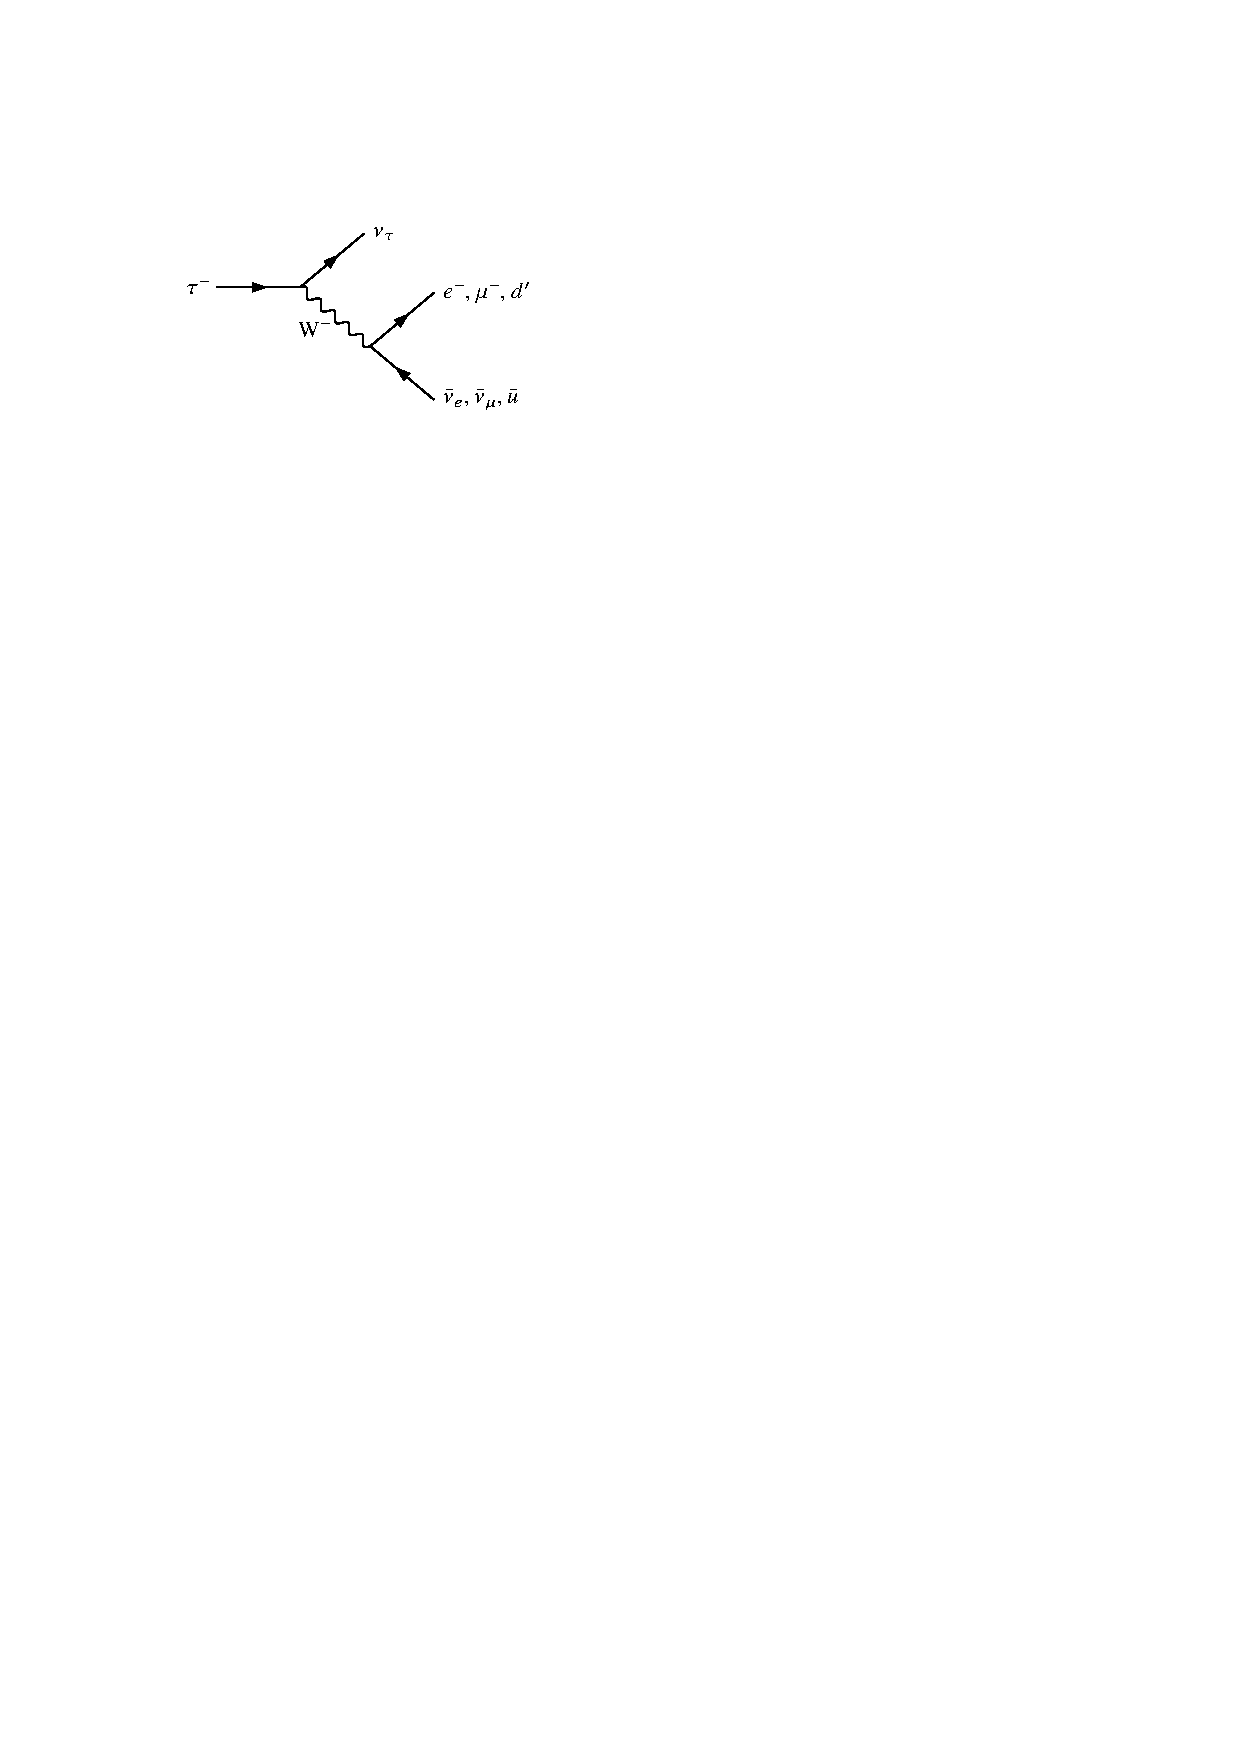
\includegraphics{figs/tauid/tau_decay_feynman}

    \vspace*{3em}
    \subcaption{a}%
    \label{fig:tau_feynman}
  \end{subfigure}\hfill
  \begin{subfigure}[b]{0.47\textwidth}
    \centering

    \begin{overpic}[scale=0.9]{figs/tauid/tau_branching_pie_chart}
      \put (31, 83) {$\pi^- \nu_\tau$}
      \put (-5.5, 45) {$\pi^- \pi^0 \nu_\tau$}
      \put (16, 7) {$\pi^- 2 \pi^0 \nu_\tau$}
      \put (40.5, 2) {$2 \pi^- \pi^+ \nu_\tau$}
      \put (65, 6.5) {$2 \pi^- \pi^+ \pi^0 \nu_\tau$}
      \put (76.5, 15.5) {other}
      \put (70, 77.5) {$e^- \bar{\nu}_e \nu_\tau$}
      \put (88.5, 41.5) {$\mu^- \bar{\nu}_\mu \nu_\tau$}
    \end{overpic}

    \subcaption{}%
    \label{fig:tau_branching_ratios}
  \end{subfigure}
  \caption{Decay and branching ratios of the tau
    lepton. Charge-conjugate decay modes are omitted.}
\end{figure}


\subsubsection{Seed Jet}

Seeded with AntiKt 0.4 jets on TopoClusters at the LC scale.

\subsubsection{Tau Vertex Association}

TJVA

\subsubsection{Track Association}

\cite{duschinger}

\todo[inline]{Make sure to point out the difference between ``tau
  tracks'' and all other tracks.}

\subsubsection{Energy Calibration}

MVA TES

\subsubsection{Electron Veto}
\subsubsection{Tau Identification}

\subsection{Missing Transverse Energy}%
\label{sec:atlas_met}


%%% Local Variables:
%%% mode: latex
%%% TeX-master: "../../phd_thesis"
%%% End:
